% ===================================================================
%  Generado por Erlen
%  Compílalo en Overleaf, o localmente con dos pasadas de pdflatex.
% ===================================================================
\documentclass[aspectratio=169,11pt]{beamer}
\usetheme{Boadilla}
% Boadilla es el tema de fábrica más limpio: sin barra de navegación.
\definecolor{acentoRevista}{HTML}{235E8C}
\setbeamercolor{structure}{fg=acentoRevista}
\usepackage[utf8]{inputenc}
\usepackage[T1]{fontenc}
% Español: se carga solo si babel-spanish está instalado (Overleaf lo trae).
\IfFileExists{spanish.ldf}{\usepackage[spanish,es-nodecimaldot]{babel}}{}
\usepackage{amsmath,amssymb}
\usepackage[version=4]{mhchem}
\definecolor{erlenacento}{HTML}{235E8C}
\usepackage{tikz}
\usetikzlibrary{arrows.meta, calc}
\usepackage{pgfplots}
\pgfplotsset{compat=1.18}
\definecolor{serieA}{HTML}{0072B2}
\definecolor{serieB}{HTML}{E69F00}
\definecolor{serieC}{HTML}{009E73}
\definecolor{serieD}{HTML}{D55E00}
\definecolor{serieE}{HTML}{CC79A7}
\definecolor{serieF}{HTML}{56B4E9}
\renewcommand{\figurename}{Figura}
\renewcommand{\tablename}{Tabla}
\usepackage{siunitx}
\sisetup{per-mode=symbol, range-units=single}
\setbeamertemplate{navigation symbols}{}
% Algunos temas (Metropolis entre ellos) insertan solos una diapositiva al
% empezar cada sección. Erlen ya emite la suya, así que se desactiva la
% automática: de otro modo cada sección saldría dos veces y la numeración
% del PDF dejaría de coincidir con la de la app.
\AtBeginSection{}
\AtBeginSubsection{}

\title[Calibración UV–Vis]{Calibración UV–Vis}
\subtitle{Ejemplo didáctico · datos ilustrativos}
\date{\today}

\begin{document}

% --- diapositiva 1 ---
\begin{frame}[plain]
  \transdissolve[duration=0.25]
  \titlepage
\end{frame}
\note{%
  {\scriptsize\textbf{Tiempo previsto: 0:30 min}}\par\medskip
  Ejemplo didáctico. Sustituye contenido y datos por los de tu trabajo. No atribuir estas cifras a un experimento.\par
}

% --- diapositiva 2 ---
\begin{frame}{La pregunta que guía el trabajo}
  \transdissolve[duration=0.25]
  {\large ¿Qué intervalo de concentración permite una calibración útil?}
  \medskip

  {\small Caso de uso ilustrativo. Define aquí el sistema, la comparación y el alcance.}
\end{frame}
\note{%
  {\scriptsize\textbf{Tiempo previsto: 1:30 min}}\par\medskip
}

% --- diapositiva 3 ---
\begin{frame}{Una estrategia explícita}
  \transdissolve[duration=0.25]
  \begin{figure}
    \centering
    \definecolor{sa0f}{HTML}{CFDCE6}
    \definecolor{sa1f}{HTML}{9DB7CC}
    \definecolor{sa2f}{HTML}{6B93B2}
    \definecolor{sa3f}{HTML}{396E98}
    \definecolor{sat1843819360}{HTML}{15181C}
    \definecolor{sat1226267613}{HTML}{FFFFFF}
    % Con babel-spanish las palabras largas se parten solas y el texto respira mejor.
    \begin{tikzpicture}[x=1cm,y=1cm,font=\footnotesize]
      \draw[fill=sa0f, draw=none] (0.000,0.000) -- (2.226,0.000) -- (2.518,-1.254) -- (2.226,-2.508) -- (0.000,-2.508) -- cycle;
      \draw[fill=sa1f, draw=none] (2.644,0.000) -- (4.870,0.000) -- (5.162,-1.254) -- (4.870,-2.508) -- (2.644,-2.508) -- (2.936,-1.254) -- cycle;
      \draw[fill=sa2f, draw=none] (5.288,0.000) -- (7.514,0.000) -- (7.806,-1.254) -- (7.514,-2.508) -- (5.288,-2.508) -- (5.580,-1.254) -- cycle;
      \draw[fill=sa3f, draw=none] (7.932,0.000) -- (10.157,0.000) -- (10.450,-1.254) -- (10.157,-2.508) -- (7.932,-2.508) -- (8.224,-1.254) -- cycle;
      \node[text=sat1843819360, align=center, text width=1.75cm, inner sep=1pt] at (1.113,-1.254) {\bfseries Preparar blancos y patrones};
      \node[text=sat1843819360, align=center, text width=1.75cm, inner sep=1pt] at (3.976,-1.254) {\bfseries Medir absorbancia};
      \node[text=sat1843819360, align=center, text width=1.75cm, inner sep=1pt] at (6.620,-1.254) {\bfseries Examinar residuos};
      \node[text=sat1226267613, align=center, text width=1.75cm, inner sep=1pt] at (9.264,-1.254) {\scriptsize \bfseries Validar con una muestra independiente};
    \end{tikzpicture}
  \end{figure}
\end{frame}
\note{%
  {\scriptsize\textbf{Tiempo previsto: 1:30 min}}\par\medskip
  Explica las decisiones y los controles, no solo los nombres de las técnicas.\par
}

% --- diapositiva 4 ---
\begin{frame}{Mostrar la evidencia}
  \transdissolve[duration=0.25]
  \begin{figure}
    \centering
    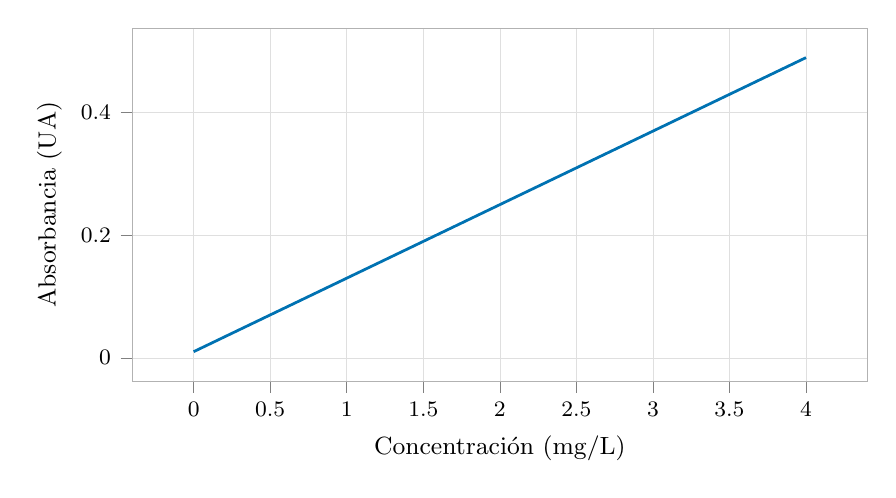
\begin{tikzpicture}
      \begin{axis}[
        width=0.90\linewidth,
        height=0.50\linewidth,
        xlabel={Concentración (mg/L)},
        ylabel={Absorbancia (UA)},
        grid=major,
        grid style={line width=.2pt, draw=gray!25},
        tick align=outside,
        tick pos=left,
        axis line style={gray!60},
        label style={font=\small},
        tick label style={font=\footnotesize}
      ]
        \addplot[serieA, line width=1pt, mark=none, smooth] coordinates {
        (0,0.01) (1,0.13) (2,0.25) (3,0.37) (4,0.49) 
        };
      \end{axis}
    \end{tikzpicture}
    \caption{Datos ilustrativos para explicar el método; sustituir por mediciones propias.}
  \end{figure}
  \medskip

  \begin{equation*}
    A = \varepsilon l c
  \end{equation*}
\end{frame}
\note{%
  {\scriptsize\textbf{Tiempo previsto: 1:30 min}}\par\medskip
  Datos o modelos didácticos: reemplazar antes de presentar resultados propios.\par
}

% --- diapositiva 5 ---
\begin{frame}{Interpretación y límites}
  \transdissolve[duration=0.25]
  \begin{itemize}
    \item Datos generados con A = 0.010 + 0.120c; no son mediciones.
    \item Una recta perfecta en datos construidos no valida un método.
    \item Sustituir por réplicas, blancos y concentraciones trazables.
  \end{itemize}
\end{frame}
\note{%
  {\scriptsize\textbf{Tiempo previsto: 1:30 min}}\par\medskip
}

% --- diapositiva 6 ---
\begin{frame}{Antes de compartir}
  \transdissolve[duration=0.25]
  \begin{itemize}
    \item Identidad del analito, disolvente y longitud de onda
    \item Unidades, incertidumbre y trazabilidad de los patrones
    \item Residuos, réplicas y validación independiente
  \end{itemize}
  \medskip

  {\small Conserva el proyecto JSON y revisa la exportación final.}
\end{frame}
\note{%
  {\scriptsize\textbf{Tiempo previsto: 1:30 min}}\par\medskip
}

\end{document}